\chapter{Active Sample Selection}
\ifpdf
    \graphicspath{{Chapter2/Chapter2Figs/PNG/}{Chapter2/Chapter2Figs/PDF/}{Chapter2/Chapter2Figs/}}
\else
    \graphicspath{{Chapter2/Chapter2Figs/EPS/}{Chapter2/Chapter2Figs/}}
\fi
\markright{\thechapter. Active Sample Selection}
\section{Background}

%\markboth{\MakeUppercase{\thechapter. My Second Chapter }}
Now that we have a good understanding of what matrix factorisation can do we focus on active learning. Typical collaborative filtering system applications are done online. This means that once a base model is learnt it evolves over time by adding new samples. For example Amazon would gradually add samples of products a user has rated, improving its model. In others contexts a research laboratory will be conducting experiments on drug-biological targets and gradually adding the results of each experiment to a database. All of these situations involve a new row-column combination being sampled. Choosing the new sample can be a matter of human judgement but cannot guarantee model improvement. Active sample selection is the process of intelligently selecting a new sample that best increases the models performance.

%\begin{figure}[!htbp]
\begin{figure}[H]
  \begin{center}
    \leavevmode
    \ifpdf
      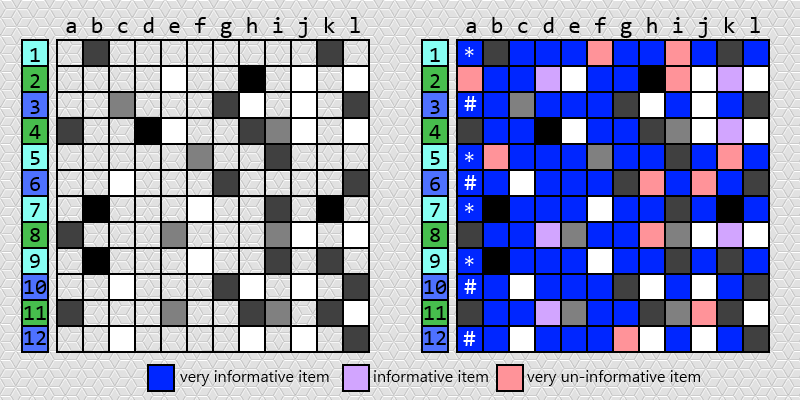
\includegraphics[width=\textwidth]{RS-ALdiag}
    \else
      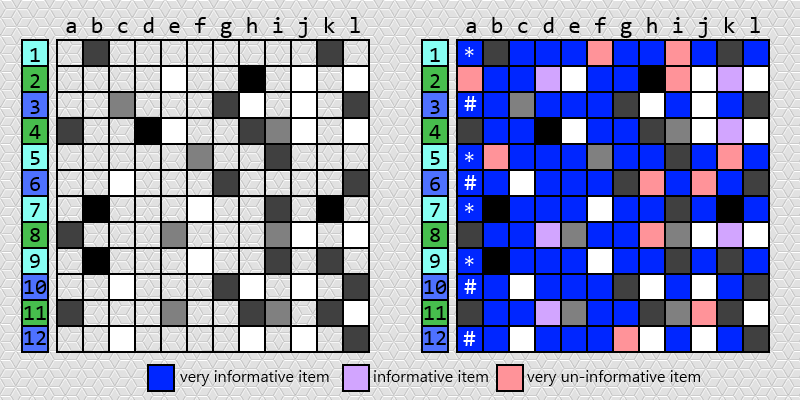
\includegraphics[bb = 92 86 545 742, width=\textwidth]{RS-ALdiag}
    \fi
    \end{center}
Users are represented in rows, and there has been 3 type of users defined, dark blue, light blue and green. Items are represented in the columns by letters. User item pairs that are rated are represented by a shade of grey and unrated squares are left blank.
    \caption{Diagram of a simplified user-item matrix used for recommender systems}
    \label{fig:al-diag}
\end{figure}

Figure \ref{fig:al-diag} gives us a very simplified graphical explanation of what an active learning system can achieve. To the left we have a sparse user-item matrix, each coloured square represents a rating, with the intensity representing a rating or interaction (for example black could represent 4, dark grey 3, light grey 2 and white 1). To simplify, we can assume that the system has recognised that there are 3 types of user groups, light blue, dark blue and green. Each of these user groups have the same interests. Using a film database analogy, a green user could be an action movie fan whereas light blue users could be comedy aficionados. Thus if it needed to predict what the rating \texttt{a2} would be, extra sampling would not really be useful as we know \texttt{a4}, \texttt{a8} and \texttt{a11}, which are all part of the green group. Knowing \texttt{a2}, along with \texttt{b5} and other pink ratings (from the right matrix) is of little use. However knowing just one of \texttt{a1-5-7-9} and \texttt{a3-6-10-12} is very useful as it gives us a rough idea as to what light and dark blue users think of item \texttt{a}. Collecting samples for users we already have a reasonably good profile of only helps us improve the certainty of certain ratings rather than be able to say something new about the dataset. Again it may be the case that the item rating isn't the same for one user group but this is an idealistic scenario.


\section{Measuring Effectiveness}
Determining whether or not a sampling method is effective or not is mainly a matter of seeing how well it impacts the performance. For example if the average sample added to a model leads to a 0.01 RMSE decrease and we can select the ones leading to 0.02 RMSE decrease on average then it can be said that this is effective. The benchmark case is defined to be random sampling, that is choosing a new sample at random. As random sampling may select an informative sample just as well as a less useful one, many random sampling trials must be done and averaged together to see the expected random performance. The benchmark RMSE for random sampling can be seen in the appendix figure \ref{fig:RandomPMF}. This is because one random sampling instance may outperform a poor active sampling method. Figure \ref{fig:al_minknowl} shows a case of random sampling performing as well or outperforming an active sampling method (in this case this is a basic one developed for this project called minimum knowledge search).

\begin{figure}[!htbp]
  \begin{center}
    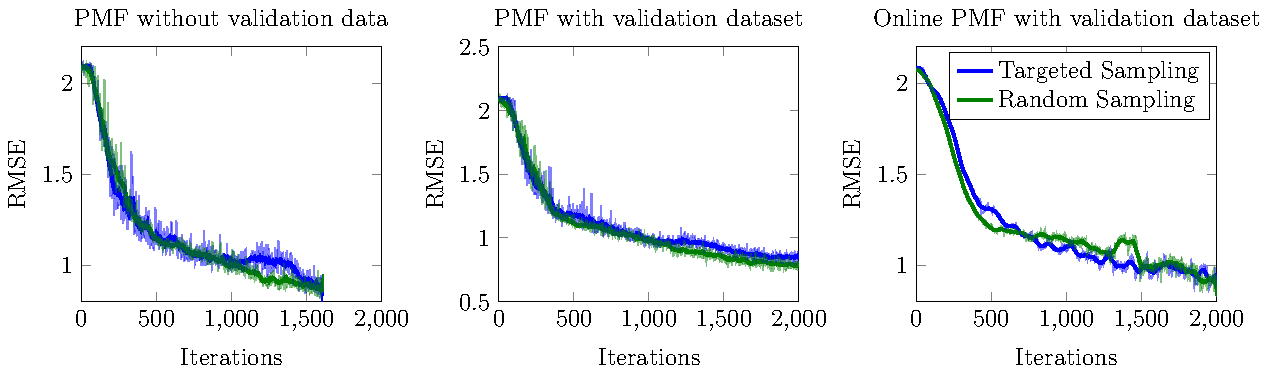
\includegraphics[width=\textwidth]{min_knowl_rate}
    Each iteration involves the discovery of one new sample. Dataset is the synthetic one from figure \ref{fig:5pcmat}.
    \caption{Active Sampling trial for the "minimum knowledge" selection}
    \label{fig:al_minknowl}
  \end{center}
\end{figure}

Another measure of the active sampling algorithm is to compare the area under the curve of the RMSE over the number of discovered samples. This measure gives an idea of what total advantage the targeted sampling may have.



It is important to be consistent with what model is used to predict data as some samples may be more useful for one model than an another. For example one model, like BPMF, will perform well by knowing a bit of everything to infer a posterior distribution of data, however PMF which does not do this will not find this sample as useful.

Effectiveness could also be linked to individual RMSE decrease, that is when a sample is discovered the amount by which it has decreased RMSE is used to rate how useful it has been. This can be a somewhat subjective error as the more about a model is know the harder RMSE decrease is.

\subsection{Discrete vs Continuous Data}
RMSE will be different for discrete and continuous data due to the way it is post-processed. Continuous data, obtained from $\hat{R}=U^TV$, is left untouched and used to calculate RMSE. For discrete data the values of $\hat{R}$ are first bounded between the minimum and maximum, for example 1 and 5 for film ratings. After this $\hat{R}$ is rounded to the nearest number in the discrete set. Error can then be calculate as traditional RMSE or as number of correct(sometimes referred to as positive) samples \cite{recsyshand}.
\section{Formal Definition}
The mask matrix $Z$ is used to determine whether a value is known (or more accurately, part of the training set, the training set mask is called $Z_{tr}$). Its indices are the same as $R$ except that values can only be $0$ or $1$. The known values are represented by $1$ and form the set $\mathcal{O}$. In other words $R_\mathcal{O}$ is the matrix of the known values. We will also have the pool of queriable samples $\mathcal{P}$, that is the samples not yet known but that may be requested. Note that it is not always the case that $R_{\mathcal{O}} \cap R_{\mathcal{P}} = R$ as there may be unqueriable unknown samples. The samples queried part of the active sampling process will form the set $\mathcal{A}$, with $R_{\mathcal{A}}$ being the requested values. In graphical form the matrix representing $\mathcal{A}$ will usually be coloured. White represents the unrequested samples and the coloured cells represent the order of sampling.


\section{Goals of Active Sampling}
\label{sec:as_goals}
To select certain samples some aspects which are thought to be able to reduce RMSE better than random selection are outlined.

\begin{description}[style=standard,leftmargin=.7cm,font=\bfseries]
  \item[Model] Look at samples that may produce the greatest change in the parameters $U$ and $V$, with he hope that this will mean a large change towards the true distribution.
  \item[Sample Uncertainty] Try to seek the samples that are most likely to vary based on current distribution of parameters, that is their uncertainty.
  \item[Knowledge] How much is known about a current row or column and aiming to maximise this overall, with the aim of getting a global insight of the data.
  \item[Max-Minimum] To best determine the boundaries of the data the largest and smallest estimated values are queried with the aim of minimising over and under estimation error.
\end{description}


\section{Minimum Knowledge Search}
\label{sec:mks_alg}
%\markboth{\MakeUppercase{\thechapter. My Second Chapter }}
Before looking at advanced sampling techniques a basic one was made to illustrate the concepts and basic increase in performance possible.
\subsection{Algorithm}
For any matrix factorisation problem we have the mask matrix $Z \in \mathbb{R}^{M \times N}$, with elements being 1 for every known value and 0 for every unknown value (values in the validation set would be also 0).

\begin{algorithm}
\caption{Minimum Knowledge Search algorithm}\label{alg:min_knowl}
\begin{algorithmic}[1]
\Procedure{MinKnowSearch}{$Z$}\Comment{The mask matrix as input}
\State $\mathbf{a} \gets \text{meanrow}(Z)$ \Comment{Mean of rows, $\mathbf{a} \in \mathbb{R}^N$}
\State $\mathbf{b} \gets \text{meancol}(Z)$ \Comment{Mean of columns, $\mathbf{b} \in \mathbb{R}^M$}
\State $K \gets \mathbf{a} \cdot \mathbf{b}$ \Comment{ $K \in \mathbb{R}^{M\times N}$}
\State $x,y \gets index\_of\_min(K)$ \Comment{Often multiple candidates, select first one}
\While{$Z(x,y)==1$}\Comment{Also check for validation mask}
\State $x,y \gets next\_min\_index(K)$
\EndWhile
\State \textbf{return} $x,y$\Comment{Return $x,y$ that has least knowledge}
\EndProcedure
\end{algorithmic}
\end{algorithm}

Knowing a bit about each column and row is a good first step to discover more about a matrix. This is the motivation of creating a heatmap of what we know about each cell. To do this we take the mean of the row and columns of $Z$. Say $\mathbf{a}=meanrow(Z)$ and $\mathbf{b}=meancolumn(Z)$. This defines the amount known for each row and column - i.e. if $\mathbf{a}_i = 0$ then there is no known sample of row $i$, if $\mathbf{b}_j = 1$ then we know all samples of column $j$. From this we can get a knowledge matrix $K= \mathbf{a} \cdot \mathbf{b}$, which acts as a heatmap of what is known of $R$. From this we can find the cells with the minimum values and target them. There will often be multiple cells of lower value but not all may be available. For example it may be impossible to sample them or it may be a cell in the validation set. For this reason we select the lowest compatible cell. The full algorithm is described in algorithm \ref{alg:min_knowl}.

\begin{figure}[!htbp]
  \begin{center}
    \resizebox{\textwidth}{!}{% This file was created by matlab2tikz v0.4.7 running on MATLAB 8.1.
% Copyright (c) 2008--2014, Nico Schlömer <nico.schloemer@gmail.com>
% All rights reserved.
% Minimal pgfplots version: 1.3
% 
% The latest updates can be retrieved from
%   http://www.mathworks.com/matlabcentral/fileexchange/22022-matlab2tikz
% where you can also make suggestions and rate matlab2tikz.
% 
\begin{tikzpicture}

\begin{axis}[%
width=2.5in,
height=2.75in,
axis on top,
scale only axis,
xmin=0.5,
xmax=50.5,
y dir=reverse,
ymin=0.5,
ymax=80.5,
name=plot2,
title={Knowledge Matrix $K$}
]
\addplot [forget plot] graphics [xmin=0.5,xmax=50.5,ymin=0.5,ymax=80.5] {search_mat-1.png};
\end{axis}

\begin{axis}[%
width=2.5in,
height=2.75in,
axis on top,
scale only axis,
xmin=0.5,
xmax=50.5,
y dir=reverse,
ymin=0.5,
ymax=80.5,
at=(plot2.left of south west),
anchor=right of south east,
title={Known Samples $Z \in \mathbb{R}^{M \times N}$}
]
\addplot [forget plot] graphics [xmin=0.5,xmax=50.5,ymin=0.5,ymax=80.5] {search_mat-2.png};
\end{axis}

\begin{axis}[%
width=.25in,
height=2.75in,
axis on top,
scale only axis,
%xmin=0.5,
%xmax=1.5,
xticklabels={,,},
%y dir=reverse,
ymin=0.5,
ymax=50.5,
name=plot3,
at=(plot2.right of south east),
anchor=left of south west
]
\addplot [forget plot] graphics [xmin=0,xmax=1,ymin=0.5,ymax=50.5] {search_mat-3.png};
\end{axis}

\begin{axis}[%
width=2.5in,
height=2.75in,
axis on top,
scale only axis,
xmin=0.5,
xmax=50.5,
y dir=reverse,
ymin=0.5,
ymax=80.5,
at=(plot3.right of south east),
anchor=left of south west,
title={Search Matrix}
]
\addplot [forget plot] graphics [xmin=0.5,xmax=50.5,ymin=0.5,ymax=80.5] {search_mat-4.png};
\end{axis}
\end{tikzpicture}%}
  \end{center}
  The darker the colour in the knowledge matrix, the least is known about that cell due to the column-row combination.
    \caption{Diagram of initial parameters and search path}
    \label{fig:min_know_search}
\end{figure}

Figure \ref{fig:min_know_search} illustrates the way minimum knowledge search works. From the known samples we see that the knowledge matrix has many "low knowledge" areas (in dark blue) to select from. A sequence of 200 sample selections is shown on the rightmost image. The first samples are blue in color, tending to red as the final samples are targeted (as shown by the colour legend to the left of it). As we see it selects the least known elements in the first row then column first. The pattern is due to selecting the very first possible least known element - a variant would be to randomly select an element to potentially try and get a temporary advantage.

\textit{Note:} Other variants of this algorithm that were tried included selecting the minimum suitable index of $\mathbf{a}$ and $\mathbf{b}$ - i.e. the coordinates that intersect with the least known row and column. However this technique did not perform as well due to not seeking to maximise one row and column first at the start. The random minimum knowledge matrix selection variant also suffers from this.


\subsection{Notes on performance}

To better compare sampling algorithms we benchmark them against random sampling by defining the advantage value as 
\begin{align*}
\frac{\text{RMSE Area under random selection}}{\text{RMSE Area under targeted selection}}
\end{align*}


\begin{figure}[!htbp]
  \begin{center}
    \resizebox{\textwidth}{!}{% This file was created by matlab2tikz v0.4.7 running on MATLAB 8.1.
% Copyright (c) 2008--2014, Nico Schlömer <nico.schloemer@gmail.com>
% All rights reserved.
% Minimal pgfplots version: 1.3
% 
% The latest updates can be retrieved from
%   http://www.mathworks.com/matlabcentral/fileexchange/22022-matlab2tikz
% where you can also make suggestions and rate matlab2tikz.
% 
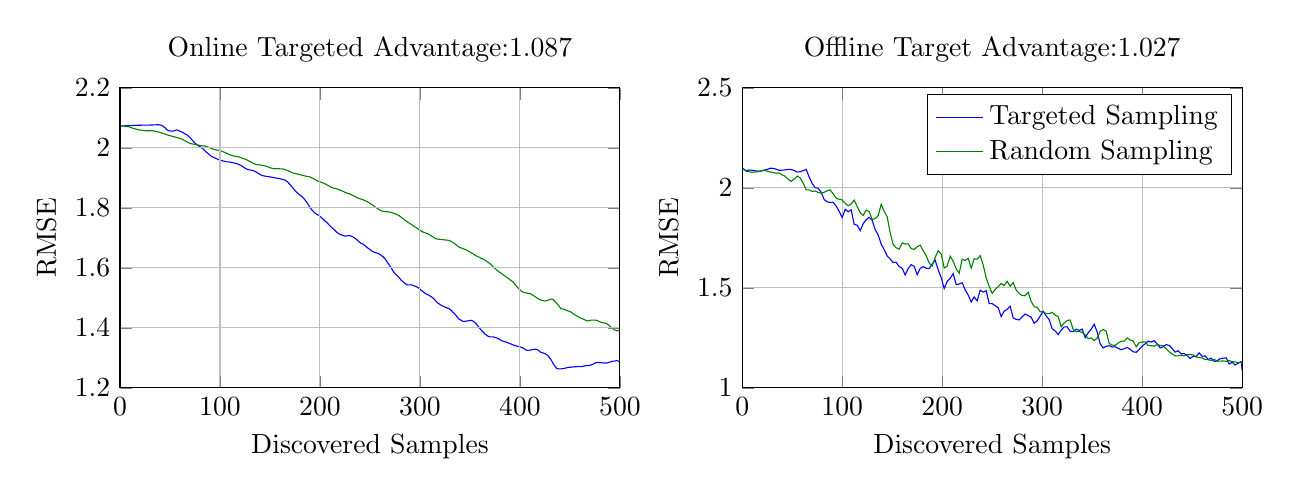
\begin{tikzpicture}

\begin{axis}[%
width=2.5in,
height=1.5in,
axis on top,
scale only axis,
xmin=0,
xmax=500,
xlabel={Discovered Samples},
xmajorgrids,
ymin=1.2,
ymax=2.2,
ylabel={RMSE},
ymajorgrids,
name=plot2,
title={Online Targeted Advantage:1.087}
]
\addplot [color=blue,solid,forget plot]
  table[row sep=crcr]{1	2.07310604133759\\
3	2.07326671713631\\
5	2.07357900586304\\
7	2.07388454435722\\
9	2.07413520970242\\
11	2.07442055079419\\
13	2.07468552217153\\
15	2.07495763872169\\
17	2.07517479065046\\
19	2.07541279796415\\
21	2.07552681878607\\
23	2.07567554770087\\
25	2.07574842378073\\
27	2.0758351989298\\
29	2.07601197081117\\
31	2.07624426489261\\
33	2.07640751446076\\
35	2.07668859545529\\
37	2.07700457165685\\
39	2.07733472347428\\
41	2.07547584678732\\
43	2.07267437054161\\
45	2.06719425000654\\
47	2.06045449193378\\
49	2.05704843627313\\
51	2.05622179611769\\
53	2.05559423696112\\
55	2.05798565857626\\
57	2.06001165822928\\
59	2.05672667279463\\
61	2.05441791887093\\
63	2.05079338565582\\
65	2.04704134065486\\
67	2.0432464385897\\
69	2.03767594564495\\
71	2.03080465916258\\
73	2.02332466132037\\
75	2.01606511084671\\
77	2.01050836397315\\
79	2.00600177919479\\
81	2.00207646759487\\
83	1.99674907672468\\
85	1.99004841108889\\
87	1.98406230282771\\
89	1.97900396970908\\
91	1.97256442314763\\
93	1.96946098036203\\
95	1.96642629748446\\
97	1.96337100951813\\
99	1.96038831260488\\
101	1.95815696385899\\
103	1.95638732161264\\
105	1.95468169501334\\
107	1.95357209186961\\
109	1.95305916135409\\
111	1.95184558004146\\
113	1.95045062137535\\
115	1.94894180782721\\
117	1.94733170690149\\
119	1.94449810032508\\
121	1.94145719906061\\
123	1.93721860458704\\
125	1.93261215856807\\
127	1.928900820703\\
129	1.92696944278035\\
131	1.92571495682112\\
133	1.92442479753473\\
135	1.9219685297118\\
137	1.91798018780745\\
139	1.91375563422737\\
141	1.90965903286238\\
143	1.90705998351704\\
145	1.905924351467\\
147	1.90459694248099\\
149	1.90378962343441\\
151	1.90281136704651\\
153	1.90115254618828\\
155	1.89997381696884\\
157	1.89896582484351\\
159	1.89769006901247\\
161	1.89642054022761\\
163	1.89480113466052\\
165	1.89259634741089\\
167	1.88858193219726\\
169	1.88140951305761\\
171	1.87415627460295\\
173	1.86647177694502\\
175	1.85775278240807\\
177	1.85127347700434\\
179	1.84584684421737\\
181	1.84002596175315\\
183	1.8346474166887\\
185	1.82673564948299\\
187	1.81786732647924\\
189	1.80720989947165\\
191	1.79704968680991\\
193	1.78919071530109\\
195	1.78254362882129\\
197	1.77865600407582\\
199	1.77449187926219\\
201	1.76918447147305\\
203	1.7629513941636\\
205	1.75651116970766\\
207	1.75149701009629\\
209	1.74332521729506\\
211	1.73676357113323\\
213	1.73087441735158\\
215	1.72489402787526\\
217	1.71814668294055\\
219	1.7135034789444\\
221	1.71056025906535\\
223	1.70786032246719\\
225	1.70594703893975\\
227	1.7064549179845\\
229	1.70807128247458\\
231	1.70605250584992\\
233	1.70312810539291\\
235	1.6988038168626\\
237	1.69329117085346\\
239	1.68705328798764\\
241	1.68182250636833\\
243	1.67963830038975\\
245	1.67427709968178\\
247	1.66841765463489\\
249	1.66358120989105\\
251	1.65840680159531\\
253	1.65381938848512\\
255	1.65120784910666\\
257	1.64960980153934\\
259	1.64719710037129\\
261	1.64236248029456\\
263	1.6372697043131\\
265	1.6305726585535\\
267	1.62103791792682\\
269	1.61081741702213\\
271	1.60121859066473\\
273	1.59010524580202\\
275	1.58088894946804\\
277	1.57515369253082\\
279	1.56853535308195\\
281	1.55984905705212\\
283	1.55345652263816\\
285	1.54825474217291\\
287	1.54366424047559\\
289	1.54334466460373\\
291	1.54360121997258\\
293	1.5417615920569\\
295	1.53934629418234\\
297	1.53640636314194\\
299	1.53194037094738\\
301	1.52632904431432\\
303	1.52108820369212\\
305	1.51562303243172\\
307	1.51160799635526\\
309	1.50891484650005\\
311	1.50422634621712\\
313	1.4997213453529\\
315	1.49290263640234\\
317	1.48500633147118\\
319	1.48039968308882\\
321	1.47551031245921\\
323	1.47218314734148\\
325	1.46942252162529\\
327	1.46682488606447\\
329	1.46401748046693\\
331	1.45893077258082\\
333	1.45211345526009\\
335	1.44610464082881\\
337	1.43769925190376\\
339	1.42911316167982\\
341	1.42586829841142\\
343	1.42174872679996\\
345	1.4214296918236\\
347	1.42332220005112\\
349	1.4236563895757\\
351	1.42534453017348\\
353	1.42321065405664\\
355	1.41751953701089\\
357	1.41054200072895\\
359	1.40219266832331\\
361	1.39329254132761\\
363	1.38637121611743\\
365	1.37964942139744\\
367	1.37478934480892\\
369	1.37057644950698\\
371	1.36980021255196\\
373	1.37016578268997\\
375	1.36849878544926\\
377	1.36600312508128\\
379	1.36317789593027\\
381	1.35855002160093\\
383	1.35561418417972\\
385	1.35344425555225\\
387	1.35185296943341\\
389	1.34882878450625\\
391	1.34627502381213\\
393	1.3436214481878\\
395	1.34098246428187\\
397	1.33921814362833\\
399	1.33820071413604\\
401	1.3354915618712\\
403	1.3330208174832\\
405	1.32868815157956\\
407	1.32484813178625\\
409	1.32507458826941\\
411	1.32664010835803\\
413	1.32798295074099\\
415	1.32903727816498\\
417	1.3282399154655\\
419	1.32359490486935\\
421	1.31842904260654\\
423	1.31639869325332\\
425	1.31414661928195\\
427	1.31018634608281\\
429	1.30341378448534\\
431	1.29460767232202\\
433	1.2821770172429\\
435	1.27232536557794\\
437	1.2645582533132\\
439	1.26313548931517\\
441	1.26337388673075\\
443	1.26431047268404\\
445	1.26546456951398\\
447	1.26725718514147\\
449	1.26876682904483\\
451	1.26885628670924\\
453	1.26961787462963\\
455	1.27037995920581\\
457	1.27068347516571\\
459	1.27078690497629\\
461	1.27083685399705\\
463	1.27166414782999\\
465	1.27345911263117\\
467	1.2741474168869\\
469	1.27434088523759\\
471	1.27651748043922\\
473	1.27875119564344\\
475	1.28247518214614\\
477	1.28468612076\\
479	1.28436084815503\\
481	1.28392412046332\\
483	1.28347928549919\\
485	1.28277225370072\\
487	1.28319989413008\\
489	1.28512421343161\\
491	1.28725828246269\\
493	1.28901363374399\\
495	1.28936602600243\\
497	1.29156219174095\\
499	1.28772549126402\\
500	1.28852400740035\\
};
\addplot [color=black!50!green,solid,forget plot]
  table[row sep=crcr]{1	2.07273486064028\\
3	2.07269718381591\\
5	2.07207773367045\\
7	2.07136282740526\\
9	2.07027448149238\\
11	2.06786230875929\\
13	2.06534441128157\\
15	2.06356333901095\\
17	2.06173328791467\\
19	2.06004227573472\\
21	2.05910548214283\\
23	2.05838424784717\\
25	2.05755798942924\\
27	2.05693269060563\\
29	2.0571709027592\\
31	2.05710941025419\\
33	2.05691498078809\\
35	2.05543771802835\\
37	2.05390367098843\\
39	2.05243943323188\\
41	2.05046108144473\\
43	2.04851158507928\\
45	2.0462022301676\\
47	2.04373646038315\\
49	2.04142481195887\\
51	2.03999919717474\\
53	2.03821157131603\\
55	2.03634853447946\\
57	2.03450626193127\\
59	2.0324709318215\\
61	2.03019705854381\\
63	2.02762814112215\\
65	2.02372983225735\\
67	2.01992164605917\\
69	2.01631269543438\\
71	2.01387316909839\\
73	2.01292768341919\\
75	2.01159687681705\\
77	2.01017193053528\\
79	2.00876764141652\\
81	2.0073175826654\\
83	2.00673400558414\\
85	2.00621494530757\\
87	2.00433376110501\\
89	2.00153619376714\\
91	1.99899125789614\\
93	1.9958294536442\\
95	1.99378977562286\\
97	1.99287231771115\\
99	1.99174488329168\\
101	1.98989301514239\\
103	1.9874859182881\\
105	1.98457721799165\\
107	1.98133411090366\\
109	1.97823871999702\\
111	1.97597888954311\\
113	1.97362908642283\\
115	1.97215187691542\\
117	1.97110251152674\\
119	1.96986189620474\\
121	1.96757155142401\\
123	1.96495689005109\\
125	1.96255143277317\\
127	1.96004569234656\\
129	1.95600702804609\\
131	1.95263731729457\\
133	1.94930393616194\\
135	1.94579517351422\\
137	1.9440219663311\\
139	1.94345924332638\\
141	1.94283532669952\\
143	1.9414643778858\\
145	1.93979929500294\\
147	1.93795540880696\\
149	1.93537415868857\\
151	1.93275895518515\\
153	1.93119726760837\\
155	1.93027734756375\\
157	1.93089373361375\\
159	1.93040045064236\\
161	1.92991454517862\\
163	1.92966004755571\\
165	1.92780129287495\\
167	1.92516480255259\\
169	1.9228116766269\\
171	1.91929104747833\\
173	1.91646847257185\\
175	1.91470426541642\\
177	1.91337976250874\\
179	1.91140772177429\\
181	1.90976391854329\\
183	1.90803981477576\\
185	1.90629695418856\\
187	1.90502081613502\\
189	1.903867372766\\
191	1.90165381329393\\
193	1.89840061356952\\
195	1.89454538088788\\
197	1.89080151856267\\
199	1.88760243532117\\
201	1.88578372128689\\
203	1.88298865851811\\
205	1.88024772260958\\
207	1.87681445170193\\
209	1.87303303950111\\
211	1.86911132960192\\
213	1.86636849750195\\
215	1.86462220722285\\
217	1.86331721169568\\
219	1.86053664743174\\
221	1.85798543831125\\
223	1.85548032151616\\
225	1.85190192536975\\
227	1.84936981877731\\
229	1.84741729078074\\
231	1.84477851681337\\
233	1.84119975342469\\
235	1.83771053918094\\
237	1.83430110402774\\
239	1.83155403929362\\
241	1.82918012653496\\
243	1.82719096966126\\
245	1.82419052244626\\
247	1.82119461975891\\
249	1.81727876511456\\
251	1.81253065789519\\
253	1.80886950779078\\
255	1.80425444679067\\
257	1.79916320501629\\
259	1.79444314818509\\
261	1.79134966250026\\
263	1.78869236256182\\
265	1.78736620048557\\
267	1.78712276571121\\
269	1.78658647730534\\
271	1.78483057407413\\
273	1.78264039788359\\
275	1.78052656980415\\
277	1.77740890983066\\
279	1.77451075306677\\
281	1.76924177249018\\
283	1.76420485369328\\
285	1.7589703598607\\
287	1.75429573859356\\
289	1.74991752472778\\
291	1.74558496165372\\
293	1.74108665583289\\
295	1.73649922694422\\
297	1.73260272536152\\
299	1.72742959923414\\
301	1.72358635766568\\
303	1.71962667584446\\
305	1.71720749911194\\
307	1.71483821299807\\
309	1.71176314116979\\
311	1.70728771832818\\
313	1.70335716048384\\
315	1.69882950335931\\
317	1.69628082535797\\
319	1.69527400934709\\
321	1.69491454482463\\
323	1.69397986357916\\
325	1.69316745473562\\
327	1.6927036066882\\
329	1.6914198932547\\
331	1.6886754428624\\
333	1.68494020500824\\
335	1.68005185496385\\
337	1.67416676625924\\
339	1.66969183991548\\
341	1.6668683040587\\
343	1.66397991920486\\
345	1.66147417376529\\
347	1.65906488942949\\
349	1.65525448066485\\
351	1.65065993029129\\
353	1.64727554951556\\
355	1.64252438564956\\
357	1.63882912730723\\
359	1.63602548617199\\
361	1.63200619424515\\
363	1.62948769076905\\
365	1.62565402111873\\
367	1.62132406834684\\
369	1.61695186847789\\
371	1.61101443180133\\
373	1.60415832438942\\
375	1.59851020796185\\
377	1.59217142296305\\
379	1.58673395734103\\
381	1.58252731088254\\
383	1.57780113026447\\
385	1.57286972547394\\
387	1.56840709394255\\
389	1.56313388791699\\
391	1.5582048828967\\
393	1.55331482357838\\
395	1.54520145783292\\
397	1.53728310651685\\
399	1.52993433356511\\
401	1.52371164110378\\
403	1.51958812343301\\
405	1.5172891526535\\
407	1.51577380981124\\
409	1.51468393953684\\
411	1.51317678444096\\
413	1.50867049372451\\
415	1.50470933432015\\
417	1.49994949606754\\
419	1.49540387377287\\
421	1.49269844866819\\
423	1.4909014464262\\
425	1.48962769543592\\
427	1.49072174272157\\
429	1.49355732074938\\
431	1.49591547834098\\
433	1.49478794974311\\
435	1.48802152015223\\
437	1.48072511194826\\
439	1.47324294134576\\
441	1.46386363227968\\
443	1.46312090117667\\
445	1.46065877443958\\
447	1.45796725612642\\
449	1.45569724049918\\
451	1.45287798998927\\
453	1.44764756061492\\
455	1.44333827238177\\
457	1.43945794536372\\
459	1.43575893140027\\
461	1.43193963415499\\
463	1.42975866882633\\
465	1.42655364396775\\
467	1.42306743343297\\
469	1.42402017484595\\
471	1.42553586963352\\
473	1.42603146555452\\
475	1.42608032701067\\
477	1.42484323113859\\
479	1.42158070572272\\
481	1.41895651444658\\
483	1.41701295189395\\
485	1.41587636236088\\
487	1.41343810856089\\
489	1.40851427344181\\
491	1.40244372478748\\
493	1.39687537335943\\
495	1.39282856164765\\
497	1.38999068219996\\
499	1.39150679218542\\
500	1.39030254853776\\
};
\end{axis}

\begin{axis}[%
width=2.5in,
height=1.5in,
scale only axis,
xmin=0,
xmax=500,
xlabel={Discovered Samples},
xmajorgrids,
ymin=1,
ymax=2.5,
ylabel={RMSE},
ymajorgrids,
at=(plot2.right of south east),
anchor=left of south west,
title={Offline Target Advantage:1.027},
legend style={draw=black,fill=white,legend cell align=left}
]
\addplot [color=blue,solid]
  table[row sep=crcr]{1	2.09623558837252\\
4	2.08557349037409\\
7	2.08941881915104\\
10	2.08810235513169\\
13	2.08528717647888\\
16	2.08368014315202\\
19	2.08349698341216\\
22	2.08898947634742\\
25	2.09236980810638\\
28	2.09796306515968\\
31	2.09777717202992\\
34	2.09303393262892\\
37	2.08777634564646\\
40	2.08852121436469\\
43	2.08995827267659\\
46	2.09256803234949\\
49	2.09169930356983\\
52	2.08658620882621\\
55	2.07945768763512\\
58	2.08068089042345\\
61	2.08621291062325\\
64	2.09258212001829\\
67	2.0542058818581\\
70	2.02210523804509\\
73	2.00033493183981\\
76	1.9981335625122\\
79	1.97872236741582\\
82	1.94140003217971\\
85	1.93060632291208\\
88	1.92687580167824\\
91	1.928208650656\\
94	1.90819705872971\\
97	1.88247183915474\\
100	1.85203041700107\\
103	1.89263828462933\\
106	1.88064430604419\\
109	1.89004831396205\\
112	1.81776837072684\\
115	1.81356653937725\\
118	1.7866644793684\\
121	1.82130467528387\\
124	1.84066550456028\\
127	1.85257625605776\\
130	1.83778378268688\\
133	1.79090500800056\\
136	1.76504190122341\\
139	1.71852334723789\\
142	1.69138855831463\\
145	1.65955104916942\\
148	1.64374996416446\\
151	1.62700545978928\\
154	1.62805841327501\\
157	1.60640282197778\\
160	1.59796309510609\\
163	1.56461229076778\\
166	1.5969255240773\\
169	1.61589295020528\\
172	1.60800140768756\\
175	1.56560748860849\\
178	1.59733589863452\\
181	1.60631219378402\\
184	1.59836503478009\\
187	1.59677922141894\\
190	1.61938847478455\\
193	1.63833230002915\\
196	1.5902394680023\\
199	1.55128520425811\\
202	1.49691177252886\\
205	1.53267550874508\\
208	1.5481229318826\\
211	1.57147425283505\\
214	1.51701589379702\\
217	1.51882054354361\\
220	1.52599256965096\\
223	1.48967665748365\\
226	1.46492482452034\\
229	1.42963487207446\\
232	1.45454414118878\\
235	1.43538311769399\\
238	1.48860176991854\\
241	1.47881243482667\\
244	1.48558190138466\\
247	1.42162604238114\\
250	1.42131112364471\\
253	1.41097835412453\\
256	1.40075480194048\\
259	1.35648946186223\\
262	1.38293641189566\\
265	1.39351226437504\\
268	1.40806431121776\\
271	1.35003740901968\\
274	1.34234875204519\\
277	1.33980333293141\\
280	1.35540243532046\\
283	1.3695812506518\\
286	1.36071571972052\\
289	1.3536985677449\\
292	1.32311148211838\\
295	1.3353322909363\\
298	1.35957413603505\\
301	1.38329491469548\\
304	1.35938035748346\\
307	1.34144645254962\\
310	1.2958979364115\\
313	1.28451415338732\\
316	1.26630672359156\\
319	1.28862354037248\\
322	1.304650178528\\
325	1.30531679354453\\
328	1.28296408867899\\
331	1.28104188752466\\
334	1.29338045409757\\
337	1.28709680143707\\
340	1.2937556124161\\
343	1.25093754566392\\
346	1.27542438464222\\
349	1.29367672538461\\
352	1.31831032055013\\
355	1.27927958090711\\
358	1.22050829708344\\
361	1.19968072447957\\
364	1.20787413555955\\
367	1.21125886047017\\
370	1.20425280652824\\
373	1.20560249522302\\
376	1.19777809597297\\
379	1.19047173137184\\
382	1.19593798976182\\
385	1.20219234974779\\
388	1.19279268203412\\
391	1.18048591479491\\
394	1.17788785225877\\
397	1.19214086630369\\
400	1.20946196406756\\
403	1.22018549445231\\
406	1.23363888661019\\
409	1.22894652874213\\
412	1.23645543338356\\
415	1.22008915667504\\
418	1.20018135249687\\
421	1.2059073531626\\
424	1.21664376577866\\
427	1.21215117662033\\
430	1.19732051507061\\
433	1.1788061330717\\
436	1.18561560279885\\
439	1.17002411488917\\
442	1.17183737388939\\
445	1.16173419562447\\
448	1.14694528339278\\
451	1.1584418315822\\
454	1.15718890613823\\
457	1.17530476412869\\
460	1.15760458870801\\
463	1.16009324205582\\
466	1.14169100000451\\
469	1.1483717150176\\
472	1.13258990901309\\
475	1.13555122302965\\
478	1.14616568657655\\
481	1.14836757627439\\
484	1.15029284211486\\
487	1.11937892444902\\
490	1.12839908103115\\
493	1.11417433212312\\
496	1.12341215670216\\
499	1.13107448027654\\
500	1.08668410908653\\
};
\addlegendentry{Targeted Sampling};

\addplot [color=black!50!green,solid]
  table[row sep=crcr]{1	2.09501172349217\\
4	2.08293870028101\\
7	2.08045379104404\\
10	2.07804993771589\\
13	2.07960926239589\\
16	2.08070758961635\\
19	2.08659654329752\\
22	2.08698059751515\\
25	2.08372191822112\\
28	2.07958988226961\\
31	2.07717778867386\\
34	2.0729447617295\\
37	2.07435901201342\\
40	2.06506462372548\\
43	2.05782756707244\\
46	2.0431666551047\\
49	2.03273931655845\\
52	2.04398815532092\\
55	2.05846140897223\\
58	2.04975864740821\\
61	2.02341162058181\\
64	1.98995433096665\\
67	1.99010890763763\\
70	1.98217891559289\\
73	1.98471274698831\\
76	1.97696137891592\\
79	1.97394935088951\\
82	1.97825743949756\\
85	1.98556259020551\\
88	1.99021035616647\\
91	1.96983766458318\\
94	1.94825841505483\\
97	1.94307209454356\\
100	1.93971453711601\\
103	1.92259485112982\\
106	1.91054335163527\\
109	1.91990824388004\\
112	1.93881315150296\\
115	1.90726268821967\\
118	1.87568821474338\\
121	1.86240064198228\\
124	1.8886402936451\\
127	1.88125116194824\\
130	1.84217791750189\\
133	1.8465042475188\\
136	1.86124269972939\\
139	1.91841606935752\\
142	1.88243201685829\\
145	1.85522441497156\\
148	1.77571870088768\\
151	1.71629539737682\\
154	1.70038322564714\\
157	1.69335511504176\\
160	1.72499588414554\\
163	1.71951511280064\\
166	1.71996542736959\\
169	1.69687223969179\\
172	1.69204457145387\\
175	1.70583018895992\\
178	1.71370884781952\\
181	1.68624132316335\\
184	1.66077403131635\\
187	1.62406406009842\\
190	1.609710112789\\
193	1.65272336588136\\
196	1.68579688066345\\
199	1.66879896851576\\
202	1.59965096673837\\
205	1.60885655719668\\
208	1.65859130548986\\
211	1.63368404741668\\
214	1.59538008534167\\
217	1.57296508833288\\
220	1.64333960214517\\
223	1.63704548741144\\
226	1.64755931922927\\
229	1.59855720305325\\
232	1.64576301295597\\
235	1.64328708688335\\
238	1.6610194350617\\
241	1.61510744865109\\
244	1.54947336430295\\
247	1.50760947759938\\
250	1.47231274285789\\
253	1.49308164602425\\
256	1.50615944196781\\
259	1.52168372612609\\
262	1.51213674885728\\
265	1.53277361500399\\
268	1.50788835084955\\
271	1.52670131041786\\
274	1.48897024187698\\
277	1.47228626179601\\
280	1.46115631482788\\
283	1.46078239963633\\
286	1.47790905368603\\
289	1.43232005406434\\
292	1.40568503277145\\
295	1.4028853987067\\
298	1.38078336394117\\
301	1.37987703280474\\
304	1.37160939503333\\
307	1.37098711603995\\
310	1.3780306759949\\
313	1.36365060159499\\
316	1.35632478725668\\
319	1.30524682081509\\
322	1.32496668875371\\
325	1.33705005462304\\
328	1.33943336108902\\
331	1.29172086141883\\
334	1.2805294706101\\
337	1.28239383509277\\
340	1.27719896562986\\
343	1.26573281850245\\
346	1.2464588393257\\
349	1.2497762588219\\
352	1.23696939355274\\
355	1.24796094031928\\
358	1.28275420364581\\
361	1.29192354645752\\
364	1.28346042815004\\
367	1.22198827043422\\
370	1.21372420348027\\
373	1.21250865874745\\
376	1.22433469913556\\
379	1.23306009853477\\
382	1.23412430492534\\
385	1.25025601339111\\
388	1.23925302577228\\
391	1.23448273107499\\
394	1.20543006731131\\
397	1.22599463503145\\
400	1.22896913685223\\
403	1.23029987714075\\
406	1.21157092252635\\
409	1.21060074776435\\
412	1.20843389564234\\
415	1.21688722820609\\
418	1.21237602156283\\
421	1.21096931775804\\
424	1.19484119909435\\
427	1.17998872640249\\
430	1.1693634680154\\
433	1.16046738879857\\
436	1.16019442991082\\
439	1.1636002745657\\
442	1.15998304862206\\
445	1.16687269643565\\
448	1.16703518583644\\
451	1.16453964363033\\
454	1.15409859651281\\
457	1.15155556156158\\
460	1.14989801984772\\
463	1.14125214893952\\
466	1.14110841823961\\
469	1.13656250413446\\
472	1.14257239295239\\
475	1.13306781671376\\
478	1.13394865406197\\
481	1.134749468441\\
484	1.13246745227602\\
487	1.13675870768403\\
490	1.13064794801889\\
493	1.13005967021843\\
496	1.12577638968963\\
499	1.12964183605538\\
500	1.12000525208853\\
};
\addlegendentry{Random Sampling};

\end{axis}
\end{tikzpicture}%}
  \end{center}
  Over 10 online trials, minimum knowledge search advantage was $1.043$. Final random RMSE:1.390, targeted RMSE:1.289.
  
   Over 10 offline trials, minimum knowledge search advantage was $1.017$. Final random RMSE:1.120, targeted RMSE:1.087. 
    
Carried out on the sample synthetic dataset with 1.25\% of samples initially discovered.  $\lambda = 0.01$, $D=7$
    \caption{RMSE vs Samples Discovered for Online PMF}
    \label{fig:online_pmf_active}
\end{figure}


Figure \ref{fig:online_pmf_active} shows the change in RMSE over time as a function of discovered samples. From this it can be seen that Minimum Knowledge Search works well on the synthetic dataset compared to random sampling, nearly always outperforming it. This is in part due to the nature of the data, which has most rows and columns containing a similar level of information that their neighbours, thus a search to find out more about the average row and column is preferred and useful. However, should most of the information only be contained in one area of the matrix then the performance would not be as satisfactory. For datasets of very low variance or uniform regions, this search could perform even better. This search method was tested on non-synthetic data, trying to recover an Eiffel Tower image, as seen in appendix figure \ref{fig:eiffel_active_mks}. As this is a somewhat uniform picture (a sky and just a structure) minimum knowledge search performed very well - 12\% advantage in this case.
\begin{figure}%
    \centering
    \subfloat[10 new samples]{{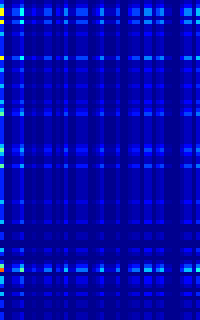
\includegraphics[width=0.25\textwidth]{know-10} }}%
    \qquad
    \subfloat[50 new samples]{{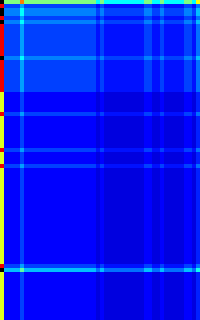
\includegraphics[width=0.25\textwidth]{know-50} }}%
    \qquad
    \subfloat[200 new samples]{{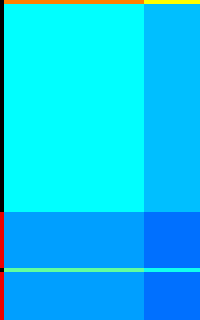
\includegraphics[width=0.25\textwidth]{know-200} }}%
    
    Knowledge scaled is same as figure \ref{fig:min_know_search} - the darker the blue the less is known.
    \caption{Evolution of Knowledge Matrix over time}%
    \label{fig:know_mat_it}
\end{figure}

The main weakness in this algorithm is described in figure \ref{fig:know_mat_it}. As it targets the row-column combinations with the least knowledge the number of samples available for selection at each step can actually increase due to the matrix becoming more uniform. Thus the potential for sample discrimination decreases over time and the advantage only exists during initial matrix sampling. Initialising a search trial with many more known samples can cause minimum knowledge search to perform 20\% worse \footnote{In terms of advantage value}.

\subsection{Comments}
The minimum knowledge search algorithm does not take the known matrix elements, nor the predicted ones, into consideration. These also contain information in themselves and could greatly help with the selection of better samples. Being dataset agnostic is an weakness of minimum knowledge search as dataset properties can greatly impact performance. For example a dataset where a row and column that has most of the less useful elements known but very useful unknown elements will not be targeted until very late on, potentially giving the random sampling an edge. Minimum knowledge search only really works on datasets where useful elements are not found in clusters.

Additionally the aim of homogenising the amount known in each column and row is not always possible in constrained situations where the sampling space is limited, that is a sample determined for selection is not available(i.e. it may not be possible to ask a user his 5 star rating of a film if he hasn't seen it).

Algorithms presented later on will take advantage of the dataset to try and get better performance.

% ------------------------------------------------------------------------

%%% Local Variables: 
%%% mode: latex
%%% TeX-master: "../thesis"
%%% End: 
